\noindent\textbf{INTRODUÇÃO}
$\!$\\
\indent Os problemas físicos de interesse da engenharia mecânica, muitas vezes, podem se apresentar de forma multidisciplinar e em razão disso também oferecem resultados que exigem ferramental e perspectivas oferecidos por outras disciplinas e áreas não contempladas em um curso usual de um engenheiro mecânico. Um desses problemas é o fenômeno de difusão acompanhado de reações químicas (homogêneas ou heterogêneas), em geral não lineares, que, em condições conhecidas, configuram processos de organização espacial de substâncias ou espécies. Por exemplo, reações químicas autocatalíticas ou outros tipos de interações em sistemas difusivos com mais de uma substâncias ou espécies, e.g., o caso particular de auto-organização dentro de uma classe mais ampla conhecida como estruturas dissipativas: padrões (estruturas) de turing.\par
\begin{figure}[H]
\centering
% 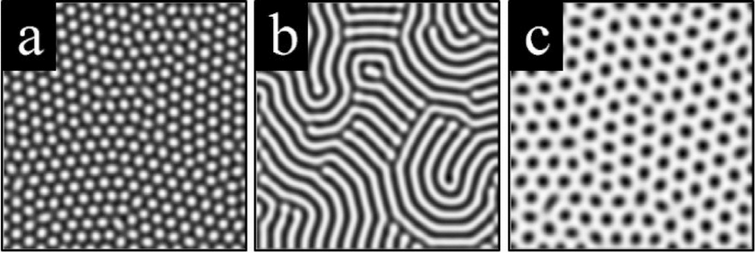
\includegraphics[scale=0.5]{01_Pre_textuais/turing2.PNG}
\end{figure}
As equações de reação-difusão são conhecidas por modelarem fenômenos químicos e biológicos, os quais, se originam da interação entre indivíduos, células ou espécies. A modelagem matemática desses mecanismos tem sido bem sucedida e vem se desenvolvendo em áreas como ecologia, embriologia (morfogênese), neurobiologia, \textcolor{red}{outros}, bem como cinéticas químicas no estado sólido. Este último tema é de interesse da ciência dos materiais computacional, uma vez que modelos matemáticos de problemas físicos tais como crescimento dendrítico (evolução cristalina), formação de precipitados em ligas metálicas e cerâmicas ou até mesmo transformação de fase por avanço de frente tornam-se possíveis.\par
Padrões espaço-temporais se apresentam em diversos âmbitos da natureza e sua descrição e compreensão ainda levantam questões importantes e básicas. Comparando com cerca de 30 anos atrás, grande progresso foi conquistado na modelagem de instabilidades, análise da dinâmica na vizinhança, formação e estabilidade de padrões, análise quantitativa experimental e numérica de padrões, e assim por diante. \par
Modelos de Reação-Difusão podem evoluir para um padrão
espacial heterogêneo e estável ao longo do tempo devido a pequenas perturbações das
concentrações das substâncias químicas em relação a um estado de equilíbrio espacial
homogêneo.\par
% Comportamentos universais de sistemas complexos próximos a instabilidades foram determinados, levando à ampla interdisciplinaridade de um campo que agora é chamado de ciência não-linear ou ciência da complexidade, e no qual conceitos iniciais de estruturas dissipativas ou sinergéticas estão profundamente enraizados.\par
% Em domínios pioneiros relacionados à hidrodinâmica ou às instabilidades químicas, as interações entre experimentalistas e teóricos, às vezes cotidianamente, têm sido fundamentais para o progresso. Todos no campo elogiam o papel desempenhado pelas interações e retornos permanentes entre estudos experimentais, numéricos e analíticos nas conquistas obtidas durante esses anos. Muitos aspectos de padrões convectivos em fluidos normais, misturas binárias ou cristais líquidos são agora entendidos e descritos neste contexto. A presença genérica de defeitos em sistemas estendidos está agora bem estabelecida e induziu novos desenvolvimentos na física de laser com grandes números de Fresnel. Por último, mas não menos importante, quase 40 anos depois de seu célebre trabalho, as estruturas de Turing foram finalmente obtidas em reatores químicos da vida real, desencadeando uma nova atividade intensa no campo dos sistemas de reação-difusão.
\textcolor{red}{Posicionar histórico, experiências, resultados, modelos, referências, etc. As teorias matemáticas...}
% \begin{figure}[H]
% \centering
% 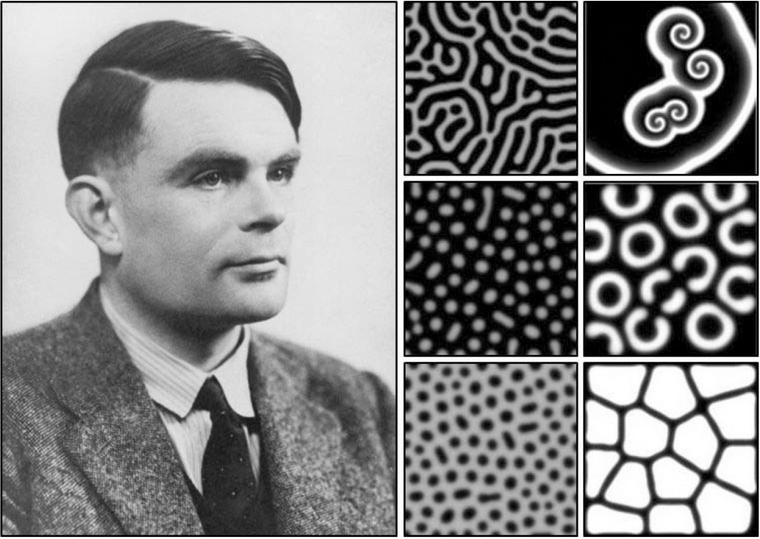
\includegraphics[scale=0.4]{01_Pre_textuais/turing1.PNG}
% \end{figure}
% \textcolor{red}{Posicionar referências}